\section{计数问题}

\title[第6讲\quad 计数问题]{第6讲\quad 计数问题} 
\author{}
\date{}

\begin{frame}
    \titlepage
\end{frame}

\setcounter{framecounter}{0}

\begin{frame}
    \stepcounter{framecounter}
    \frametitle{习题\theframecounter}
    \textit{如图,2x3的棋盘上由6个单位正方形构成,棋盘上共有12 个格点,甲、乙、丙、丁11.
四人站在其中四个格点上,若任意两人处于同一横线或竖线则认为可相互看见。
甲说:我可以看见你们所有人。
乙说:我一个人也看不到。
丙说:我只能看到一个人。
丁说:我们四人所在格点连成四边形面积为3,且任意3人所在格点组成的三角形面积都不为整数。
已知四人中看见人数最多(其他人看见的人数都比他看见的少)的那个人说了假话,其他人都说了真话,那么这4人有\underline{\hbox to 20mm{}}种不同的站法.}
    \begin{figure}[H] 
        \centering
        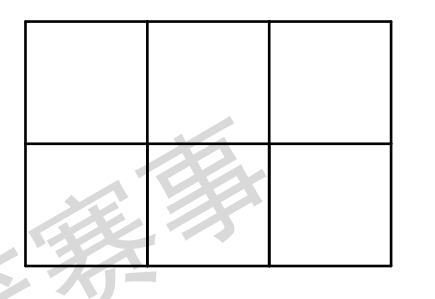
\includegraphics[width=0.4\textwidth]{./pics/Chapter_6/1.png}
    \end{figure}
    % 2025;8
\end{frame}


\begin{frame}
    \stepcounter{framecounter}
    \frametitle{习题\theframecounter}
    \textit{如图所示,墙上挂着6件礼物,分成两列,每列必须从下往上依次取走。现在有6位同学,身高分别为 100、120、140、160、180、200厘米.每人只能拿到最多比自己身高高 100 厘米处的礼物.现在6位同学排成一列拿取礼物.为了让每人都能拿到一件礼物,有\underline{\hbox to 20mm{}}种符合要求的排队方式.}
    \begin{figure}[H] 
        \centering
        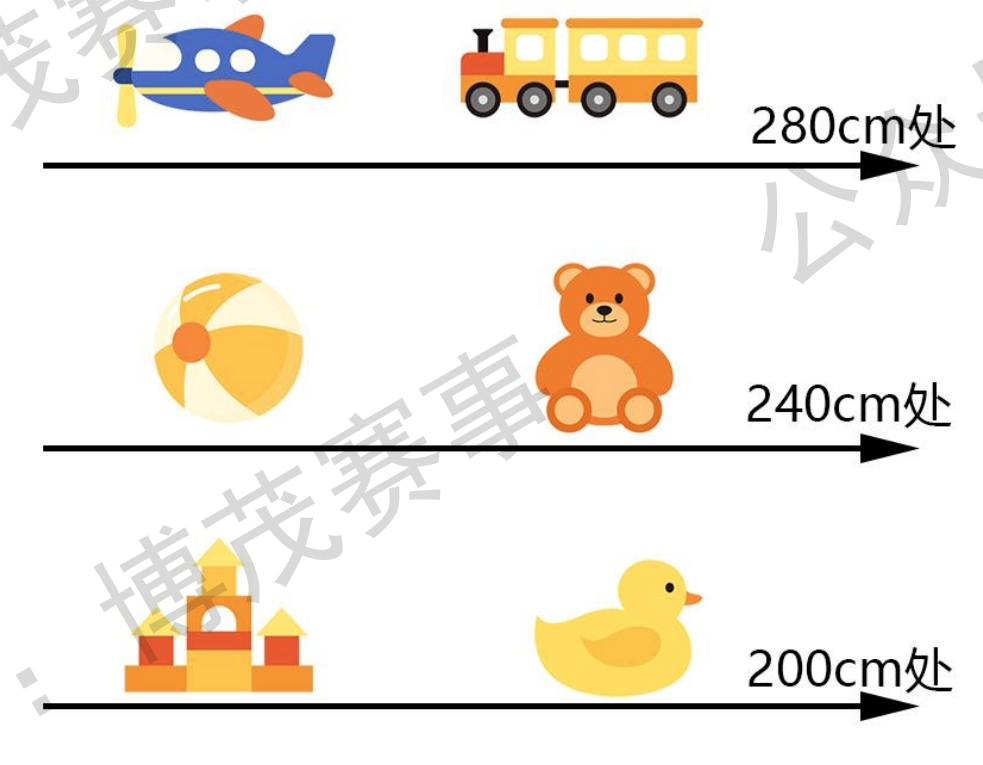
\includegraphics[width=0.4\textwidth]{./pics/Chapter_6/2.png}
    \end{figure}
    % 2025;40
\end{frame}

\begin{frame}
    \stepcounter{framecounter}
    \frametitle{习题\theframecounter}
    \textit{如图所示,墙上挂着6件礼物,分成两列,每列必须从下往上依次取走。现在有6位同学,身高分别为 100、120、140、160、180、200厘米.每人只能拿到最多比自己身高高 100 厘米处的礼物.现在6位同学排成一列拿取礼物.为了让每人都能拿到一件礼物,有\underline{\hbox to 20mm{}}种符合要求的排队方式.}
    \begin{figure}[H] 
        \centering
        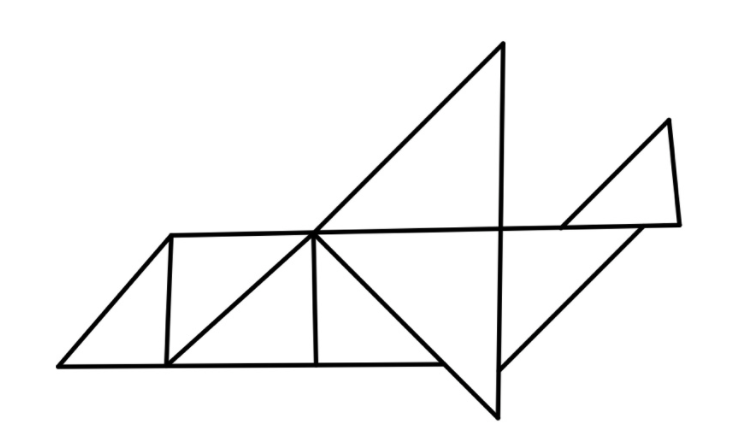
\includegraphics[width=0.4\textwidth]{./pics/Chapter_6/3.png}
    \end{figure}
    % 2025;40
\end{frame}


\begin{frame}
    \stepcounter{framecounter}
    \frametitle{习题\theframecounter}
    \vspace*{-3cm}
    \textit{将1、2、3、4、5、6、7、8这八个数字分别填到一个固定好的正方体的八个顶点上,要求同一条棱上的两个数之和小于12,那么共有\underline{\hbox to 20mm{}}种不同的填法.}
    % 2024;
\end{frame}


\begin{frame}
    \stepcounter{framecounter}
    \frametitle{习题\theframecounter}
    \vspace*{-1cm}
    \textit{图中,三角形共有\underline{\hbox to 20mm{}}个.}
    \begin{figure}[H] 
        \centering
        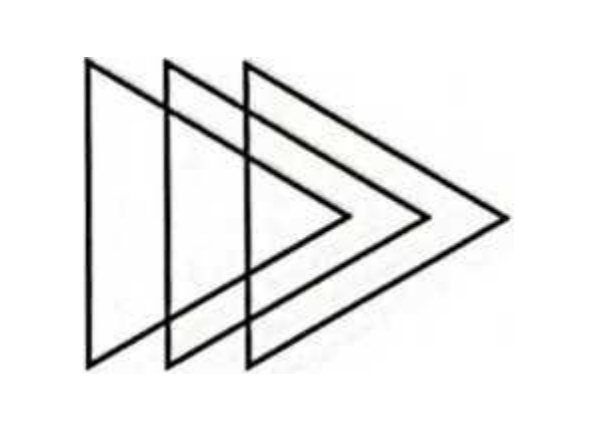
\includegraphics[width=0.4\textwidth]{./pics/Chapter_6/5.png}
    \end{figure}
    % 2023;6
\end{frame}

\begin{frame}
    \stepcounter{framecounter}
    \frametitle{习题\theframecounter}
    \textit{右图已固定,请将1、2、3、4各两个分别填入八个圆圈中,使得阴影圆圈中的数比它两边相邻的白色圆圈中的数都大;那么不同的填法共有\underline{\hbox to 20mm{}}种.}
    \begin{figure}[H] 
        \centering
        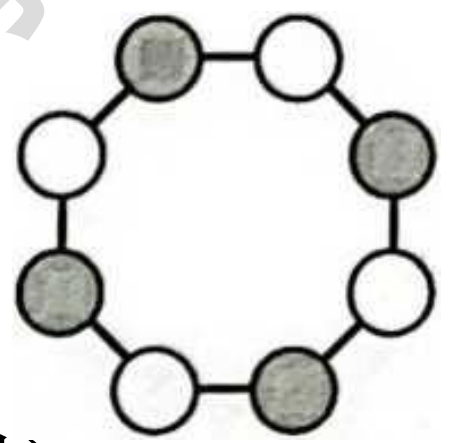
\includegraphics[width=0.4\textwidth]{./pics/Chapter_6/6.png}
    \end{figure}
    % 2023;44
\end{frame}

\begin{frame}
    \stepcounter{framecounter}
    \frametitle{习题\theframecounter}
    \vspace*{-1cm}
    \textit{右图中共能数出\underline{\hbox to 20mm{}}个 三角形.}
    \begin{figure}[H] 
        \centering
        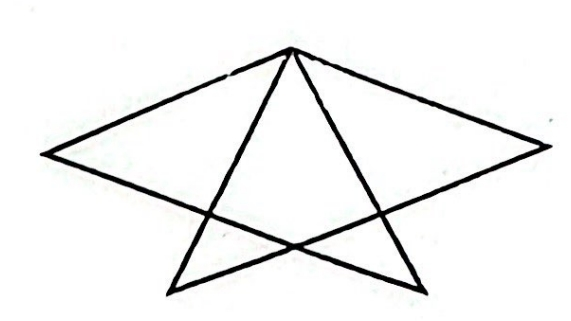
\includegraphics[width=0.4\textwidth]{./pics/Chapter_6/7.png}
    \end{figure}
    % 2024;8
\end{frame}


\begin{frame}
    \stepcounter{framecounter}
    \frametitle{习题\theframecounter}
    \textit{如图,在正方体的一些顶点处各有一只蚂蚁,它们的爬行速度相同且只能沿着正方体的棱爬行,在棱上爬行到达下一个顶点前不能回头,且从未有任两只蚂蚁相遇.\\
    (1)如果在 A、B 处各有一只蚂蚁,每只蚂蚁各爬行1条棱,共有\underline{\hbox to 10mm{}}种不同的爬行情况.\\
    (2)如果在 A、C、F 处各有一只蚂蚁,每只蚂蚁各爬行2条棱, 
    一共有 \underline{\hbox to 10mm{}} 种不同的爬行情况.
    }
    \begin{figure}[H] 
        \centering
        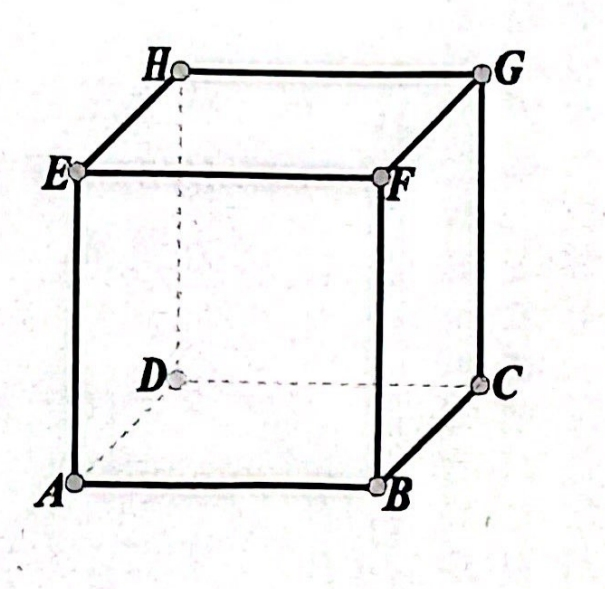
\includegraphics[width=0.2\textwidth]{./pics/Chapter_4/2.png}
    \end{figure}
    % 2023. 8;121
\end{frame}


\begin{frame}
    \stepcounter{framecounter}
    \frametitle{习题\theframecounter}
    \vspace*{-1cm}
    \textit{下左图是由“开罗五边形”组成的拼接图,图中的每个五边形的形状大小完全相同,观察图形并确定下右图中的图形在下左图中共出现了 \underline{\hbox to 10mm{}} 次.(右图图形可以旋转观察)}
    \begin{figure}[H] 
        \centering
        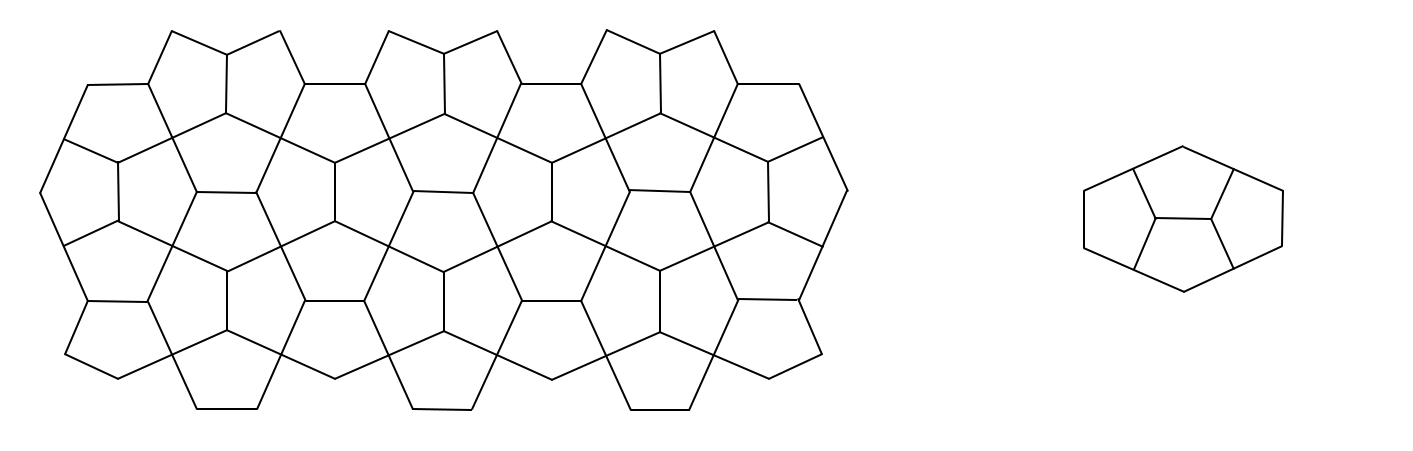
\includegraphics[width=0.8\textwidth]{./pics/Chapter_6/8.png}
    \end{figure}
    % 2023. 8;121
\end{frame}

\begin{frame}
    \stepcounter{framecounter}
    \frametitle{习题\theframecounter}
    \vspace*{-1cm}
    \textit{丽丽想用大小为 1x1、2x2、3x3的三种正方形拼成下图所示的领奖台(图中每个小正方形的边长为1),所用正方形的面积总和为 15,且拼接过程中不可重叠,每种正方形数量不限(可以不用).共有 \underline{\hbox to 10mm{}} 种不同的拼接方法.(正方形的摆放位置或数量不同都算不同的拼法)}
    \begin{figure}[H] 
        \centering
        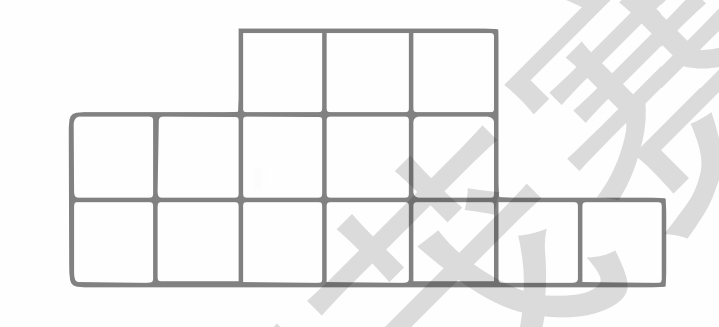
\includegraphics[width=0.6\textwidth]{./pics/Chapter_6/9.png}
    \end{figure}
    % 2022
\end{frame}

\begin{frame}
    \stepcounter{framecounter}
    \frametitle{习题\theframecounter}
    \vspace*{-3cm}
    \textit{老师手中有4张牌,按照甲、乙、甲、乙的顺序分发。如果这4张牌的点数分别是 1、2、3、4,并且在整个过程中(包括最终),甲手中牌的点数之和一直比乙大,那么,满足要求的分发顺序共有 \underline{\hbox to 10mm{}} 种.}
    % 2022
\end{frame}

\begin{frame}
    \stepcounter{framecounter}
    \frametitle{习题\theframecounter}
    \textit{右图中,共有 \underline{\hbox to 10mm{}} 个三角形.}
    \begin{figure}[H] 
        \centering
        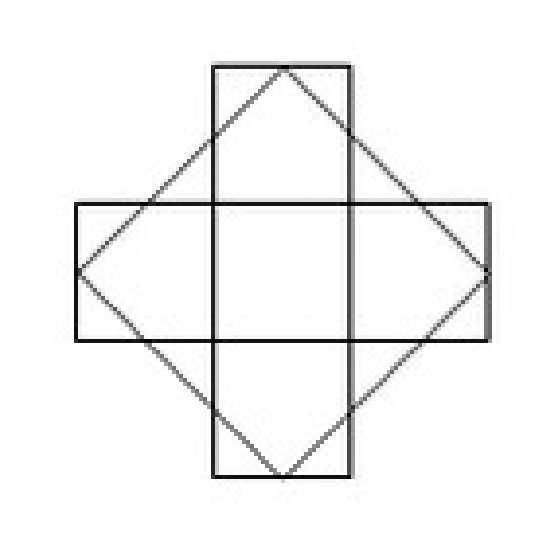
\includegraphics[width=0.5\textwidth]{./pics/Chapter_6/12.png}
    \end{figure}
    % 2021;16
\end{frame}

\begin{frame}
    \stepcounter{framecounter}
    \frametitle{习题\theframecounter}
    \textit{如右图,小鱼老师在为圣诞树准备装饰物,每个树顶需要放一颗幸运星每一层树的两侧需要各放1个许原球,一共3层,小鱼老师数了数,许愿球比幸运星多 40个,那么,小鱼老师装饰了 \underline{\hbox to 10mm{}} 棵圣诞树.}
    \begin{figure}[H] 
        \centering
        
\includegraphics[width=0.3\textwidth]{./pics/Chapter_6/13.png}
    \end{figure}
    % 2021;8
\end{frame}


\begin{frame}
    \stepcounter{framecounter}
    \frametitle{习题\theframecounter}
    \textit{右图中,共有 \underline{\hbox to 10mm{}} 个正六边形.}
    \begin{figure}[H] 
        \centering
        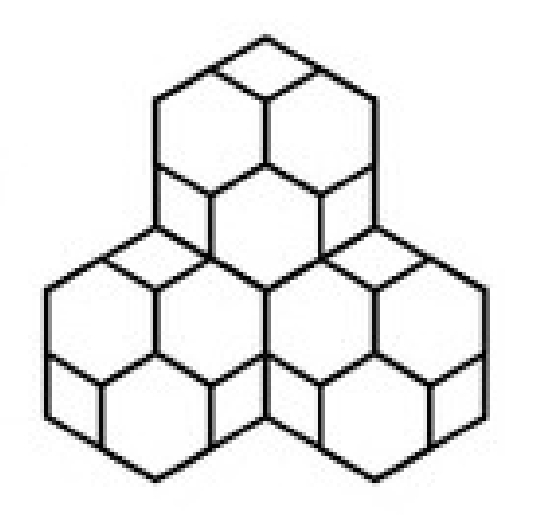
\includegraphics[width=0.4\textwidth]{./pics/Chapter_6/14.png}
    \end{figure}
    % 2021;12
\end{frame}

\begin{frame}
    \stepcounter{framecounter}
    \frametitle{习题\theframecounter}
    \textit{如图,一个 的正方体六个面已经被染成了不同的六种颜色.现将其分成4个 的小长方体,共有\underline{\hbox to 10mm{}}种不同分法.}
    \begin{figure}[H] 
        \centering
        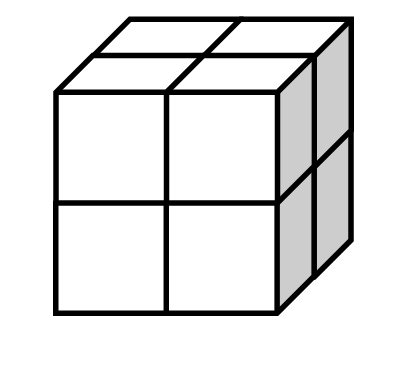
\includegraphics[width=0.4\textwidth]{./pics/Chapter_6/15.png}
    \end{figure}
    % 2020;9
\end{frame}